\section{简谐振动的几何表述}\label{sec:07.03}

为了进一步理解简谐振动\lhbrak 式\eqref{eqn:07.02.04}\rhbrak 的特性,我们再来研
究匀速圆周运动。如图\ref{fig:07.06}\;表示一个以$ r _ { 0 } $为半径的圆周运动。若角
速率为恒定的,则按\ref{sec:01.09}\,节中的表示可知,质点的角位置$ \varphi $与角速
率$ \omega $的关系为:
\begin{equation}\label{eqn:07.03.01}
  \varphi = \omega t + \varphi _ { 0 }
\end{equation}
式中$ \varphi _ { 0 } $是$ t = 0 $时刻的角位置。

\begin{figure}[h]
  \centering
  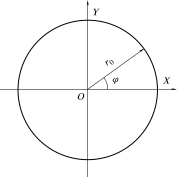
\includegraphics{figure/fig07.06}
  \caption{圆周运动与简谐振动}
  \label{fig:07.06}
\end{figure}

如果我们用$ \left(x, y\right) $坐标来描写质点的位置则有
\begin{equation}\label{eqn:07.03.02}
  \begin{aligned}
    x & = r _ { 0 } \cos \varphi \\
    y & = r _ { 0 } \sin \varphi
  \end{aligned}
\end{equation}
将式\eqref{eqn:07.03.01}代入式\eqref{eqn:07.03.02},得到
\begin{equation*}
  x = r _ { 0 } \cos \left( \omega t + \varphi _ { 0 } \right)
\end{equation*}
\begin{equation}\label{eqn:07.03.03}
  y = r _ { 0 } \sin \left( \omega t + \varphi _ { 0 } \right)
\end{equation}
对比式\eqref{eqn:07.03.03}及式\eqref{eqn:07.02.04},可见两者是完全相同的,只是式
\eqref{eqn:07.02.04}中的振幅$ A $在式\eqref{eqn:07.03.03}中变成了$ r _ { 0 } $。因此,结论是:匀速
圆周运动质点的$ x $坐标按简谐振动方式变化。

\begin{wrapfigure}[6]{r}{14em}
  \vspace{-0.8em}
  \centering
  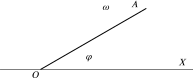
\includegraphics{figure/fig07.07}
  \caption{简谐振动的几何表述}
  \label{fig:07.07}
\end{wrapfigure}
这个结果启发我们可以把每个简谐振动用一个匀速
圆周运动来表述。如图\ref{fig:07.07},如果简谐振动是沿着$ X $轴
的,那么我们可以用矢量$ \vec{ OA } $
来代表这个简谐振动。$ \vec{ OA } $
的长度等于简谐振动的振幅,它以匀角速率$ \omega $绕$ O $转动。$ \vec{ OA } $与
$ X $轴的夹角$ \varphi $,就是位相。矢量$ \vec{ OA } $在$ X $轴上的投影即为振子的
位置坐标,这种表述简谐振动的方法称为几何表述。
